\documentclass[12pt]{article}
\usepackage{amsfonts, amssymb, amsmath, amsthm}
\usepackage[margin=1in]{geometry}
\usepackage{tikz}
\usetikzlibrary{patterns, decorations.pathreplacing}

\pagestyle{myheadings}
\markright{Explainer: Kuratowski's Closure-Complement Problem\hfill}

\newcommand{\R}{\mathbb{R}}

\begin{document}

\begin{center}
    \textbf{\Large The Kuratowski Closure-Complement Problem}\\[0.5em]
    \large Understanding the two operations
\end{center}

\section*{The Problem}

\begin{quote}
\textit{Consider the collection of all subsets of a topological space. The operations of taking closure and complement produce at most 14 sets. Show this and give an example of a subset of the reals that produces exactly 14 sets.}
\end{quote}

\section{The Two Operations}

We have two operations we can apply to any subset $A$ of a topological space $X$:

\subsection{Complement: $A^c$}

The \textbf{complement} $A^c = X \setminus A$ consists of all points \emph{not} in $A$.

\begin{center}
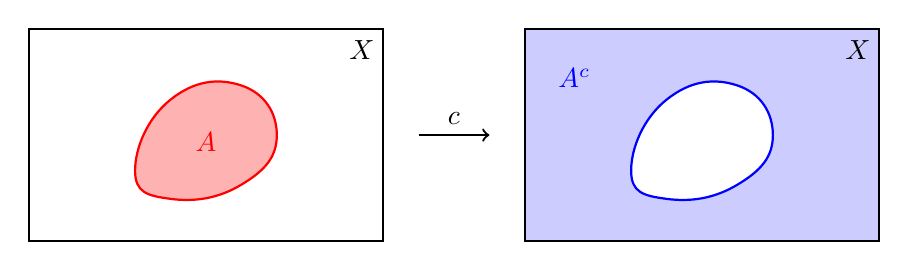
\begin{tikzpicture}[scale=0.9]
    % The space X
    \draw[thick] (0,0) rectangle (5,3);
    \node at (4.7, 2.7) {$X$};

    % Set A
    \fill[red!30] plot[smooth cycle, tension=0.8] coordinates {(1.5,1) (2,2) (3,2.2) (3.5,1.5) (3,0.8) (2,0.6)};
    \draw[red, thick] plot[smooth cycle, tension=0.8] coordinates {(1.5,1) (2,2) (3,2.2) (3.5,1.5) (3,0.8) (2,0.6)};
    \node[red] at (2.5, 1.4) {$A$};

    \draw[->, thick] (5.5, 1.5) -- (6.5, 1.5) node[midway, above] {$c$};

    % After complement
    \begin{scope}[xshift=7cm]
        \fill[blue!20] (0,0) rectangle (5,3);
        \fill[white] plot[smooth cycle, tension=0.8] coordinates {(1.5,1) (2,2) (3,2.2) (3.5,1.5) (3,0.8) (2,0.6)};
        \draw[thick] (0,0) rectangle (5,3);
        \draw[blue, thick] plot[smooth cycle, tension=0.8] coordinates {(1.5,1) (2,2) (3,2.2) (3.5,1.5) (3,0.8) (2,0.6)};
        \node at (4.7, 2.7) {$X$};
        \node[blue] at (0.7, 2.3) {$A^c$};
    \end{scope}
\end{tikzpicture}
\end{center}

\textbf{Key property:} $(A^c)^c = A$ \quad (complementing twice gives back the original)

\subsection{Closure: $\overline{A}$}

The \textbf{closure} $\overline{A}$ is the smallest closed set containing $A$. Equivalently, $\overline{A} = A \cup A'$ where $A'$ is the set of limit points.

\begin{center}
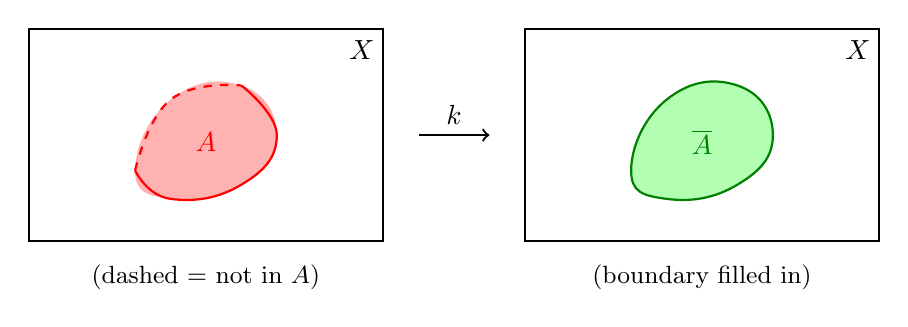
\begin{tikzpicture}[scale=0.9]
    % Original set (open interval style)
    \draw[thick] (0,0) rectangle (5,3);
    \node at (4.7, 2.7) {$X$};

    % Set A (with some boundary missing)
    \fill[red!30] plot[smooth cycle, tension=0.8] coordinates {(1.5,1) (2,2) (3,2.2) (3.5,1.5) (3,0.8) (2,0.6)};
    \draw[red, thick, dashed] plot[smooth, tension=0.8] coordinates {(1.5,1) (2,2) (3,2.2)};
    \draw[red, thick] plot[smooth, tension=0.8] coordinates {(3,2.2) (3.5,1.5) (3,0.8) (2,0.6) (1.5,1)};
    \node[red] at (2.5, 1.4) {$A$};
    \node at (2.5, -0.5) {\small (dashed = not in $A$)};

    \draw[->, thick] (5.5, 1.5) -- (6.5, 1.5) node[midway, above] {$k$};

    % After closure
    \begin{scope}[xshift=7cm]
        \draw[thick] (0,0) rectangle (5,3);
        \fill[green!30] plot[smooth cycle, tension=0.8] coordinates {(1.5,1) (2,2) (3,2.2) (3.5,1.5) (3,0.8) (2,0.6)};
        \draw[green!50!black, thick] plot[smooth cycle, tension=0.8] coordinates {(1.5,1) (2,2) (3,2.2) (3.5,1.5) (3,0.8) (2,0.6)};
        \node at (4.7, 2.7) {$X$};
        \node[green!50!black] at (2.5, 1.4) {$\overline{A}$};
        \node at (2.5, -0.5) {\small (boundary filled in)};
    \end{scope}
\end{tikzpicture}
\end{center}

\textbf{Key property:} $\overline{\overline{A}} = \overline{A}$ \quad (closure is idempotent---closing twice is the same as closing once)

\section{The Game: Apply Operations Repeatedly}

Starting with any set $A$, we can keep applying closure ($k$) and complement ($c$):

\begin{center}
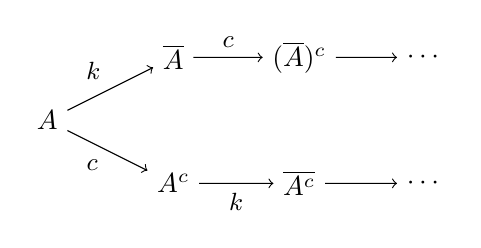
\begin{tikzpicture}[scale=0.8]
    \node (A) at (0,0) {$A$};
    \node (kA) at (2,1) {$\overline{A}$};
    \node (cA) at (2,-1) {$A^c$};
    \node (ckA) at (4,1) {$(\overline{A})^c$};
    \node (kcA) at (4,-1) {$\overline{A^c}$};
    \node (dots1) at (6,1) {$\cdots$};
    \node (dots2) at (6,-1) {$\cdots$};

    \draw[->] (A) -- (kA) node[midway, above left] {\small $k$};
    \draw[->] (A) -- (cA) node[midway, below left] {\small $c$};
    \draw[->] (kA) -- (ckA) node[midway, above] {\small $c$};
    \draw[->] (cA) -- (kcA) node[midway, below] {\small $k$};
    \draw[->] (ckA) -- (dots1);
    \draw[->] (kcA) -- (dots2);
\end{tikzpicture}
\end{center}

\textbf{The Question:} How many \emph{distinct} sets can we produce this way?

\section{Why Not Infinitely Many?}

At first, it seems like we could get infinitely many sets by alternating operations forever. But the key properties limit us:

\begin{itemize}
    \item $c \circ c = \text{id}$ (complement twice = do nothing)
    \item $k \circ k = k$ (closure twice = closure once)
\end{itemize}

So we never need two $c$'s in a row, and we never need two $k$'s in a row.

This means every sequence of operations can be written as an alternating sequence:
\[ k, \quad c, \quad kc, \quad ck, \quad kck, \quad ckc, \quad kckc, \quad ckck, \quad \ldots \]

\textbf{But even this doesn't obviously stop!} The claim is that this process eventually stabilizes after at most 14 distinct sets.

\section{The Two Parts of the Problem}

\textbf{Part 1:} Prove that starting from \emph{any} set in \emph{any} topological space, applying closure and complement repeatedly produces \textbf{at most 14} distinct sets.

\textbf{Part 2:} Find a specific subset of $\R$ (with usual topology) that achieves \textbf{exactly 14} distinct sets.

\section{What Makes a Set ``Interesting''?}

For a set to produce many distinct sets under these operations, it needs to have interesting structure. Consider:

\begin{center}
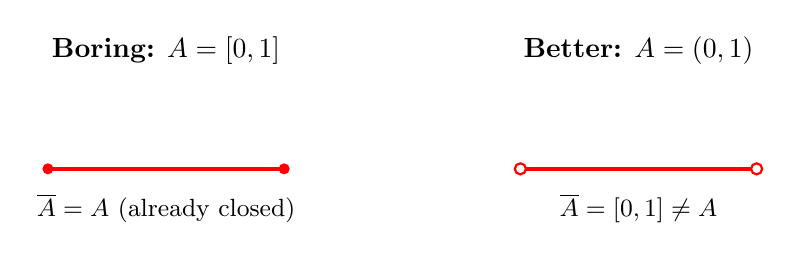
\begin{tikzpicture}[scale=1]
    % Boring example: closed interval
    \begin{scope}
        \node at (1.5, 1.5) {\textbf{Boring:} $A = [0,1]$};
        \draw[very thick, red] (0,0) -- (3,0);
        \fill[red] (0,0) circle (2pt);
        \fill[red] (3,0) circle (2pt);
        \node at (1.5, -0.5) {\small $\overline{A} = A$ (already closed)};
    \end{scope}

    % More interesting: open interval
    \begin{scope}[xshift=6cm]
        \node at (1.5, 1.5) {\textbf{Better:} $A = (0,1)$};
        \draw[very thick, red] (0,0) -- (3,0);
        \draw[red, thick, fill=white] (0,0) circle (2pt);
        \draw[red, thick, fill=white] (3,0) circle (2pt);
        \node at (1.5, -0.5) {\small $\overline{A} = [0,1] \neq A$};
    \end{scope}
\end{tikzpicture}
\end{center}

To get many sets, you want $A$ where:
\begin{itemize}
    \item $A \neq \overline{A}$ (not closed)
    \item $A^c \neq \overline{A^c}$ (complement not closed)
    \item The pattern keeps producing new sets for as long as possible
\end{itemize}

\section{Notation Shorthand}

It's convenient to write $k$ for closure and $c$ for complement:
\begin{align*}
    kA &= \overline{A} \\
    cA &= A^c \\
    kcA &= \overline{A^c} \\
    ckA &= (\overline{A})^c
\end{align*}

The 14 sets (when all distinct) come from applying these operators in all possible alternating patterns.

\end{document}
